% http://www.ctan.org/tex-archive/macros/latex/contrib/beamer/examples
% http://latex.artikel-namsu.de/english/beamer-examples.html

%\documentclass{beamer}
\documentclass[usenames,dvipsnames,12pt,compress]{beamer}
\setbeamertemplate{navigation symbols}{}
\usepackage{amsmath}
\usepackage{amssymb}
\usepackage{bm}
\usepackage{fancybox, graphicx}
\usepackage{listings}
\usepackage{tikz} % Diagrams
\usetikzlibrary{positioning}
\usepackage{color}
\usepackage{textcomp} % See https://tex.stackexchange.com/questions/145416/how-to-have-straight-single-quotes-in-lstlistings
%\usepackage[font=small,labelfont=bf]{caption} % Required for specifying captions to tables and figures. From https://tex.stackexchange.com/questions/238636
\usepackage[absolute,overlay]{textpos}


\lstset{language=bash,upquote=true} % Format listings as appropriate for bash. Inexplicably we get problems if the language is set as part of the \begin{lstlisting} command.

% https://tex.stackexchange.com/questions/36030/how-to-make-a-single-word-look-as-some-code
\definecolor{light-gray}{gray}{0.95}
\newcommand{\code}[1]{\colorbox{light-gray}{\texttt{#1}}}

\newcommand{\mentiurl}[0]{{\url{www.menti.com}}}
\newcommand{\menticode}[0]{{9850 5737}}
\newcommand{\mentiinvitation}[0]{Go to \mentiurl{} (code \menticode{}) and choose one possibility:\\}
\newcommand{\correctanswer}[1]{\textcolor{blue}{{#1} \checkmark}}

% Parameters: file name, graphics options (e.g. `scale=0.3'), whom to credit, x pos for credit, y pos for credit.
\newcommand{\imageandcredit}[5]{
  {
    \begin{tikzpicture}
      \draw (-4, 0) node[inner sep=0] {\includegraphics[{#2}]{{#1}}};
      \draw ({#4},{#5}) node[white,fill=black,font=\footnotesize] {Credit: {#3}};
    \end{tikzpicture}
  }
}

% Parameters: file name, graphics options (e.g. `scale=0.3'), background colour, whom to credit, x pos for credit, y pos for credit.
\newcommand{\framewithimageandcredit}[6]{
{
  \setbeamercolor{background canvas}{bg={#3}}
  \begin{frame}{}
    \begin{center}
      \imageandcredit{#1}{#2}{#4}{#5}{#6}
    \end{center}
  \end{frame}
 }
}

% Parameters: file name, graphics options (e.g. `scale=0.3'), background colour
\newcommand{\framewithimage}[3]{
{
  \setbeamercolor{background canvas}{bg={#3}}
  \begin{frame}{}
    \begin{center}
      \begin{tikzpicture}
        \draw (0, 0) node[inner sep=0] {\includegraphics[{#2}]{{#1}}};
      \end{tikzpicture}
    \end{center}
  \end{frame}
 }
}

%Parameters: Item text, file name, graphics options, credit
\newcommand{\itemandimageandcredit}[4]{
  \begin{columns}
  \column{0.04\linewidth}
  \column{0.41\linewidth}
  \item{#1}
  \column{0.55\linewidth}
  \imageandcredit{#2}{#3}{#4}{-4}{-1.3}
  \end{columns}
}


%\usetheme{boxes}
%\usecolortheme{beaver}


\title{The Constantly Changing Hubble Constant}
\author{Lorne Whiteway \\ lorne.whiteway@star.ucl.ac.uk}
\institute{Astrophysics Group \\ Department of Physics and Astronomy \\ University College London}
\date{Presentation to the Mid Kent Astronomical Society \\ 12 November 2021 \\ Find the presentation at \alert{\url{https://tinyurl.com/bycke8v6}}}

\begin{document}

\frame{\titlepage}


\begin{frame}{Interactive content}
  \begin{block}{}
    You are invited to go to\\
    \begin{center}
    \huge \alert{\mentiurl{}}\\
    \end{center}
    and enter code\\
    \begin{center}
    \huge \menticode{}
    \end{center}
  \end{block}
\end{frame}


\begin{frame}{The Universe is expanding!}
  \begin{block}{}
  \begin{itemize}
  \item{But what does this actually mean?}
  \item{How do we know it is expanding?}
  \item{Why is it expanding?}
  \item{How fast is it expanding?}
  \item{Are cosmologists completely realistic about the uncertainties in their results?}
  \end{itemize}
  \end{block}
\end{frame}

\begin{frame}{How do we know?}
  \begin{columns}
    \column{0.4\linewidth}
    \begin{itemize}
    \item{Everywhere we look, distant galaxies are receding; more distant galaxies are receding faster.}
    \item{So either we are at the centre of a cosmic conspiracy, or all the space between all the galaxies is expanding.}
    \end{itemize}
    \column{0.6\linewidth}
    \centering
    % https://en.wikipedia.org/wiki/Hubble_Ultra-Deep_Field#/media/File:Hubble_ultra_deep_field_high_rez_edit1.jpg
    \imageandcredit{720px-Hubble_ultra_deep_field_high_rez_edit1.jpg}{height=7cm}{NASA Ultra Deep Field}{-5}{-3.2}
  \end{columns}
\end{frame}

\begin{frame}{Is the solar system expanding? Are \textit{we} expanding?}
  \begin{block}{}
    \mentiinvitation{}
    \begin{enumerate}
      \item{Yes, a lot}
      \item{Yes, but only a tiny amount}
      \item{No}
    \end{enumerate}
  \end{block}
\end{frame}

\begin{frame}{Is the solar system expanding? Are \textit{we} expanding?}
  \begin{block}{}
    \mentiinvitation{}
    \begin{enumerate}
      \item{Yes, a lot}
      \item{Yes, but only a tiny amount}
      \item{\correctanswer{No}}
    \end{enumerate}
  \end{block}
\end{frame}

\begin{frame}{Is the solar system expanding? Are \textit{we} expanding?}
  \begin{block}{}
    \begin{itemize}
      \item{Other forces - molecular forces between the molecules in your body, and gravitational forces between the Sun and the planets - are far more than strong enough to overcome the effect of cosmic expansion.}
    	% https://creativecommons.org/licenses/by-sa/4.0/deed.en
    	% https://upload.wikimedia.org/wikipedia/commons/thumb/8/8c/Andromeda_Galaxy_560mm_FL.jpg/1024px-Andromeda_Galaxy_560mm_FL.jpg
      \itemandimageandcredit{Gravity is even strong enough to keep the Andromeda Galaxy from receding from us.}{Andromeda_Galaxy_560mm_FL.jpg}{height=2.5cm}{David Dayag}
	\item{It's only the furthest objects - where gravity becomes negligible - that recede.}
    \end{itemize}
  \end{block}
\end{frame}

\begin{frame}{What does \textit{recession velocity} actually mean?}
  \begin{block}{}
  \begin{itemize}
  \item{We say `distant galaxies are moving away from us'. This is informal language.}
  \item{They aren't really moving, they just appear to be - because the intervening space is expanding.}
  \item{Sometimes this makes a difference - for example, the recession velocity can exceed the speed of light.}
  \end{itemize}
  \end{block}
\end{frame}

\begin{frame}{So how fast is the expansion?}
  \begin{block}{}
  \begin{itemize}
  \item{For every additional distance of one megaparsec, there's an additional recession velocity of about 70 kilometers per second.}
  \item{So the expansion speed is about 70 kilometers per second per megaparsec.}
  \item{One megaparsec is about three million light years. It's the typical distance between galaxies.}
  \item{70 kilometers per second is about 150,000 miles per hour.}
  \end{itemize}
  \end{block}
\end{frame}

\begin{frame}{So how fast is the expansion?}
    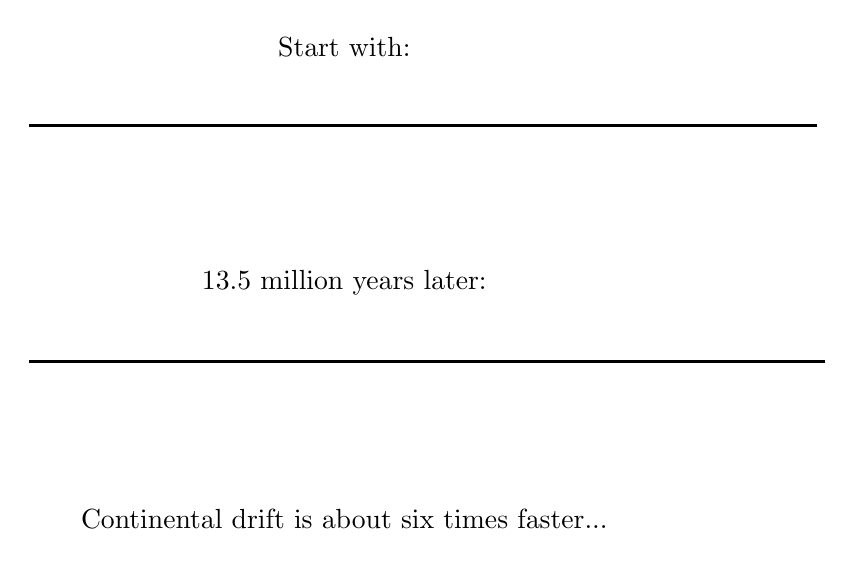
\begin{tikzpicture}
    \node at (4,1) {Start with:};
    \draw [very thick] (0,0)--(10,0);
    \pause
    \node at (4,-2) {13.5 million years later:};
    \draw [very thick] (0,-3)--(10.1,-3);
    \pause
    \node at (4,-5) {Continental drift is about six times faster...};
    \end{tikzpicture}
\end{frame}


\begin{frame}{$H_0$}
  \begin{block}{}
  \begin{itemize}
  \item{The expansion rate is denoted `$H_0$'.}
  \bigskip
  % Image of Hubble from https://commons.wikimedia.org/wiki/File:Studio_portrait_photograph_of_Edwin_Powell_Hubble.JPG
  % Johan Hagemeyer (1884-1962), Public domain, via Wikimedia Commons
  \itemandimageandcredit{The `$H$' commemorates Edwin Hubble (1889-1953), who was one of the first to measure it.}{Studio_portrait_photograph_of_Edwin_Powell_Hubble.jpg}{height=3cm}{Johan Hagemeyer}
  \bigskip
  \item{The `$0$' refers to today. The expansion rate was different in the distant past.}
  \end{itemize}
  \end{block}
 \end{frame}



% Image of Hubble from https://commons.wikimedia.org/wiki/File:Studio_portrait_photograph_of_Edwin_Powell_Hubble.JPG
\framewithimageandcredit{Studio_portrait_photograph_of_Edwin_Powell_Hubble.jpg}{angle=0,origin=l,scale=0.15}{black}{Johan Hagemeyer (1884-1962), Public domain, via Wikimedia Commons}{-4}{-3}



\end{document}
